\documentclass[12pt]{article}

\usepackage{sbc-template}
\usepackage{graphicx,url}
\usepackage[utf8]{inputenc}
\usepackage[brazil]{babel}
\usepackage{float}

\usepackage{indentfirst} % SBC nao usa indentfirst, mas acho melhor com identacao

\title{Multi-nuvem}

\author{Alexandre Canalle\inst{1}, Ariel Frozza\inst{1}}

\address{Instituto de Informática -- Universidade Católica do Paraná (PUC-PR)\\
	Caixa Postal 15.064 -- 91.501-970 -- Curitiba -- PR -- Brazil
	\email{arielfrozza@gmail.com, roxsnd@gmail.com}
}

\begin{document}

\sloppy
\maketitle
	
\begin{abstract}
	This meta-paper describes the style to be used in articles and short papers
	for SBC conferences. For papers in English, you should add just an abstract
	while for the papers in Portuguese, we also ask for an abstract in
	Portuguese (``resumo''). In both cases, abstracts should not have more than
	10 lines and must be in the first page of the paper.
\end{abstract}

\begin{abstract} 
	Neste trabalho exploraremos os conceitos de Multi-Cloud e Infrastructure as Code, bem como suas possíveis utilizações em ambientes corporativos. Também descreveremos as dificuldades na implementação de Multi-Cloud e elencaremos possíveis soluções para as dificuldades descritas.  Por fim, apresentaremos um roteiro de uso das ferramentas OpenSource Terraform e Ansible para demonstrar a implementação de um serviço web em duas Nuvens simultaneamente, uma pública (AWS) e uma privada (Openstack).
\end{abstract}

	\section{Introdução}
	    Atualmente, o uso simultâneo de serviços e recursos de múltiplos provedores de Nuvem é justificado pela necessidade de seus consumidores, expressas em requerimentos tais como qualidade de serviço e custo. As organizações que estão migrando para a Nuvem, seja para estender ou substituir sua infraestrutura \textit{on-premises}, buscam soluções confiáveis, seguras e, se possível, sem aprisionamento à fornecedores ou soluções fechadas (\textit{vendor lock in}).
	    
	    Este artigo pretende descrever alguns desafios do uso simultâneo de mais de um provedor de Nuvem e levantar alguns dor principais pontos de atenção na utilização das atuais soluções que buscam atender as necessidades dos usuários de múltiplas Nuvens. Primeiramente, a definição e a necessidade de um ambiente em Multi-nuvem é discutida, em seguida, um modelo padrão de arquitetura para Multi-nuvem é apresentado. A partir desta arquitetura de referência, algumas soluções (software) que tornam possíveis a Infraestrutura como Código em Multi-nuvem são apresentados e discutidos. Por último, ilustraremos, a partir de um exemplo prático (disponível em https://github.com/arielfrozza/multi-cloud) os processos, requisitos e desafios na implementação de IaaS em Multi-nuvem usando ferramentas e princípios típicos de Infraestrutura como Código.
	    
	    Este artigo não apresenta abordagem inovadora, entretanto, ele intenta apontar algumas lacunas e dificuldades a serem sanadas por desenvolvedores e usuários de ambientes em Multi-nuvem. Em especial, discutiremos \textit{frameworks} e padrões de provisionamento em Nuvem (pública, privada ou híbrida) que ofereçam APIs que disponibilizam funcionalidades compatíveis ou equivalentes com os softwares,  serviços e APIs ofertados pelos principais provedores de Nuvem, de modo que o provisionamento, orquestração e uso de vários provedores de Nuvens diferentes seja facilitado.
		
	\section{Definição e Necessidade de Multi-nuvens}
	
		\subsection{Infraestrutura como Código}
	
	Infraestrutura como código – IaC (Infrastructure as Code) é o processo de gerenciamento e provisionamento de recursos de infraestrutura através de código e arquivos de configuração que descrevem o estado desejado para os recursos de infraestrutura. IaC usa definições declarativas ao invés de processos manuais ou procedurais. Como se tratam de arquivos de código, as definições podem ser armazenadas em um sistema de controle de versões, tal como o Git.
	
	Algumas vantagens da utilização de IaC incluem a \textbf{eliminação de tarefas repetitivas} possibilitando a  \textbf{fácil replicação de implementações} quando o bloco de código pode ser executado repetidas vezes, fazendo poucas modificações (ou nenhuma em alguns casos) para criar ou modificar recursos em diferentes ambientes (Produção, Teste, Desenvolvimento) Nuvens (GCP, Azure ou AWS por exemplo). Uma vez que a infraestrutura  está codificada de forma estruturada e geralmente em módulos, o código pode ser \textbf{reaproveitado}. O fato da infraestrutura estar definida toda em código, e este estar \textbf{versionado} em ferramentas como Git, possibilita \textbf{maior controle nas aplicações de mudança} nos ambientes possibilitando, inclusive, a \textbf{recuperação de desastres}. O versionamento do código em Git, também possibilita a simplificação da \textbf{documentação do código}, bem como sua \textbf{manutenção e suporte}. Além disso, com IaC, fica fácil utilizar-se das mesmas técnicas de \textbf{planejamento e testes automatizados} há muito tempo utilizadas por desenvolvedores.	
	
	Nuvens podem ser usadas de forma serial, por exemplo, quando migramos de uma Nuvem para outra, ou de forma simultânea, quando usamos recursos de duas ou mais Nuvens diferentes ao mesmo tempo. O senário mais comum para o caso de uso simultâneo é a Nuvem Híbrida, quando alguns serviços são disponibilizados a partir de uma Nuvem (Privada) e outros serviços estão em uma Nuvem Pública.
	
	Os motivos que justificam o uso de múltiplas Nuvens são inúmeros e dependem da natureza do negócio de cada usuário, mesmo assim é possível citar algumas vantagens do uso simultâneo de dois ou mais provedores de Nuvem:
	
	\textbf{Tolerância à falhas} (fault-tolerance) ao envolver uso de mais de um provedor de Nuvem simultaneamente, permitindo movimentações de contingência no caso de indisponibilidade de um dos provedores, por exemplo.
	
	\textbf{Neutralidade de fornecedor} possibilita a implementação de IaaS e/ou PaaS nos principais provedores de Nuvens usando soluções diversas (em especial \textit{open-source}) evitando o aprisionamento à um fornedor (\textit{vendor lock-in}).
	
	\textbf{Performance} ao possibilitar ajustes nos níveis de carga para outros provedores de Nuvem em caso de degradação de performance ou qualidade de serviço em um dos provedores.
	
	\textbf{Segurança} TODO
	
	\textbf{Eficiência de custos} como abilidade de aproveitar os melhores preços de recursos computacionais e serviços em um ambiente Nulti-nuvem.
	
	Os custos de operação em um determinado provedor Nuvem variam em função dos requisitos de uso e da época de contratação dos serviços assim como os custos de trocar de provedor podem ficar muito altos caso a infraestrutura e/ou aplicações tenham que ser refeitos/revistos inteiramente. Por exemplo, um dos modelos de compra de VMs da Amazon, o AWS Spot Instance, oferece descontos para certos casos de uso, que podem chegar a 90\%, quando sua infraestrutura encontra-se ociosa. Outro exemplo é reflexo da redução dos custos operacionais dos provedores de Nuvem ao longo do tempo. De 2011 para 2013, ocusto por hora do AWS EC2 baixou cerca de 30\% \cite{Golden:2013}. Com o uso de padrões \textit{vendor neutral}, o objetivo seria ser capaz de mudar de provedor de cloud ou priorizar a execução \textit{on-premises} de acordo com a conveniência, sem ter que alterar o \textit{software stack}.
	
	Muitos termos são encontrados na literatura para designar o uso simultâneo de duas ou mais Nuvens. A citar os mais recorrentes \cite{Ferrer:2012}; Multi-cloud, Cloud-federation, Inter-cloud, Hybryd Cloud, Cloud of Clouds, Sky Computing, Aggregated Clouds, Fog Computing, Distributed Clouds, etc.
	
	Sendo assim, achamos útil delimitar o conceito de Multi-nuvem abordado neste artigo de outros modelos de uso combinado de Nuvens.
	
	De acordo com \cite{Ferrer:2012}, temos dois modelos de entraga de serviços em múltiplas Nuvens; Nuvem Federada e Multi-nuvem (\textit{Federated Cloud} e \textit{Multi-Cloud}). A diferença entre estes modelos seria o grau de colaboração entre os provedores de Nuvem e pelo modo pelo qual os usuários interagem com as Nuvens. No primero modelo há o acordo de uso compartilhado dos recursos entre os provedores de Nuvem. Os usuários de uma Nuvem federada não ficam sabendo, na maioria dos casos, de qual dos provedores um determinado recurso está sendo consumido. No caso do Multi-nuvem, o usuário está ciente e é responsável pela alocação de recursos em um ou outro provedor e não há nuência dos provedores para uso compartilhado de recursos entre os provedores.
	
	Sky Computing, Aggregated Clouds, Multi-tier Clouds ou Cross-Cloud são casos particulares de Nuvens Federadas e portanto não serão abordadas neste artigo. 
	
	O tipo mais comum de Multi-nuvem é a Nuvem Híbrida na qual involve duas ou mais Nuvens, por exemplo, uma Nuvem Privada e uma Pública. Comumente, esse modelo de Nuvem Híblrida é usado para transbordo de capacidade (\textit{cloud bursting}) onde os recursos são expandidos para a Nuvem Pública quando os recursos da Nuvem privada chegam nos níveis máximos pré-definidos \cite{Ferrer:2012}. A migração de uma Nuvem para outra, mesmo que apenas uma vez, é outro exemplo de uso de (one-time) Multi-nuvem.
	
	A interoperabilidade entre os diversos serviços ofertados e orquestração de recursos em múltiplas Nuvens (usando Infraestrutura como Código \cite{Morris:2016}, por exemplo) ainda está distante da maturidade, já que, por exemplo, todos os provedores de Nuvens experimentam, eventualmente, períodos de indisponibilidade que podem causar impactos a negócios \cite{Fisher:2018}. Também pode ser um problema a performance variável quando os provedores de Nuvem fazem a oversubscrição (\textit{overprovision}) da sua infraestrutura virtualizada e isto resulta em degradação de performance e qualidade de serviço \cite{CloudSpectator:2017}. Outro ponto importante é que a maioria dos provedores de Nuvem  (inclusive os líderes de mercado) disponibilizam Software e APIs proprietárias, que não são aderentes à padrões de \textit{Cloud API} como propostos por OASIS TOSCA \cite{TOSCA:2019} ou OASIS CAMP \cite{CAMP:2019}.
	 
	A seguir descreveremos um framework para o uso de Multi-nuvem envolvendo duas Nuvens, uma Privada e outra Pública. 
	
	
	
	\section{Arquitetura de Referência para Multi-nuvem}
	
	A seguir exploramos um padrão de implementação de Multi-nuvem, conforme ilustrado na Figura1, que propõem ajudar a atender dois casos comuns de uso de multi-nuvem:
	
	\textbf{Trasnbordo para Nuvem Pública} (\textit{Busting Pattern}): em algumas situações, a capacidade \textit{on-premises} de uma empresa pode exaurir e pode-se querer usar a capacidade em uma Nuvem pública para suprir uma determinada demanda.
	
	\textbf{Alta Disponibilidade}: eventualmente, um provedor de Nuvem pode ficar (parcial ou totalmente) indisponível ou com degradação na qualidade dos serviços por diversos motivos, pode-se querer migrar de um provedor para outro os serviços e recursos para não impactar o usuário final. Por exemplo, em caso de falha ou manutenção do datacenter que hospeda a Nuvem privada, pode-se migrar serviços para uma Nuvem pública, mesmo que temporariamente.
	   
	\textbf{Eficiência de Custos}: em alguns casos, provedores oferecem descontos ou modificam seus preços em função da oferta e demanda, pode-se migrar uso de recursos e serviços de uma Nuvem para outra sem que o usuário final seja impactado.
	
	A [Figura 1] ilustra as atividades e processos envolvidos para atingir os objetivos descritos acima. Outros benefícios, tais como Tolerância à Falhas, Segurança, Validação experimental, etc, também podem ser alcançados usando este mesmo padrão ou após serem feitas pequenas modificações, os quais não serão diretamente abordados neste artigo, mas podem ser entendidos de forma mais completa em \cite{Fisher:2018}.
		
	\begin{figure}[H]
		\centering
		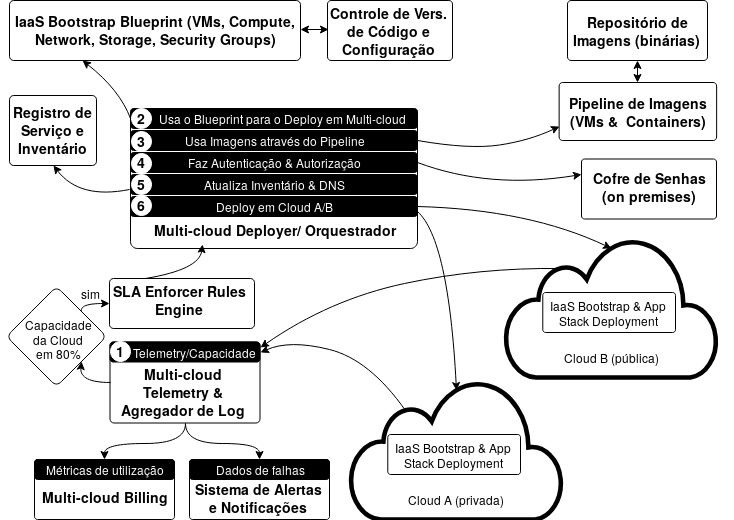
\includegraphics[width=0.9\linewidth]{figuras/Figure1.png}
		\caption{legenda longa figura1}
		\label{fig:figure1}
	\end{figure}
	
	Está numerada na Figura1 a ordem do processo de provisionamento de recursos em Multi-nuvem, que inicia em \textbf{Multi-cloud Telemetry (1)} coma coleta e agregação dados de capacidade das Nuvens integrantes da Multi-nuvens. Na Figura1 estão representadas uma Nuvem Privada e outra Publica, mas poderiamos expandir essa mesma arquitetura para um conjunto maior de diferentes provedores. As informações coletadas são repassadas para o \textbf{SLA Enforcer Rules Engine}, que valida a condição para a migração de recursos de uma Nuvem para outra, como exemplo, se a capacidade de uma das Nuvens chegar a 80\%, faz-se deploy de novos recursos apenas na outra Nuvem. O \textbf{SLA Enforcer Rules Engine} pode avaliar um conjunto de condições que se faça adequado para cada negócio ou situação, por exemplo ele pode avaliar condições de custo ou tempo de resposta, além da capacidade. A avaliação deste processo dispara o gatilho para iniciar as novas implementações através do \textbf{Multi-nuvem Deployer/Orquestrator}. Além disso, o \textbf{Multi-nuvem Telemetry \& Log Aggregator}, também gera subsídio para a bilhetagem através de métricas de utilização que são contabilizadas e disponibilidadas para o usuário através do processo \textbf{Multi-cloud Billing}. Também os alertas de erros são tratados e processados pelo processo \textbf{Sistema de Alertas e Notificações}.
	
	\textbf{Multi-nuvem Deployer/Orquestrator} \textbf{(2)} e \textbf{(3)} utiliza as definições de implementações armazenadas como código em texto em controle de versão, Git por exemplo. Estas definições de implementações são aplicadas sobre as imagens selecionadas do \textbf{Pipeline de Imagens} binárias que podem ser VMs (em formato OVA, VMDK, VHD ou RAW por exemplo) ou Containers (Docker, por exemplo).
	
	Toda informação sensível, em especial senhas ou chaves são obtidas do \textbf{Cofre de Senhas} \textbf{(4)}, que por motivos de segurança e de facilidade de acesso, geralmente está on premises e não em uma das Nuvens que fazem parte da Multi-nuvem.   
	
	Os serviços e itens de configuração ativos são registrados no \textbf{Registro de Serviços e Inventário (5)}, bem como o DNS é atualizado para refletir os novos registros e rotas.
	
	Alguns componentes do \textbf{Cloud Deployer/Orquestrator (6)} criam os componentes definidos nas etapas anteriores em cada uma das Nuvens especificadas usando as APIs de cada fornecedor. Os softwares usados nesta etapa do Cloud Deployer devem possuir uma camada de abstração das diversaas APIs para que a implementação seja o mais transparente possível e que os códigos envolvidos possam ser reaproveitados e não sejam complexos, ou difíceis de manter e documentar (alguns softwares serão apresentados e demosntrados na seção a seguir).  

	O cenário descrito acima inicia em \textbf{Telemetry (1)}, assim possibilitando situações automatizadas de orquestração dos recursos na Multi-nuvem, entretanto, um humano também poderia iniciar esse processo, passando instruções diretamente ao processo \textbf{Multi-cloud Deployer/Orquestrator}.  
	
	Os processos descritos acima e esquematizados na Figura1 podem ser bastante complexos e envolver outros subprocessos e também um conjunto diversificado de ferramentas e softwares. Como exemplo, exploremos em mais detalhes o \textbf{Pipeline de Imagens}.
		
    \begin{figure}[H]
    	\centering
    	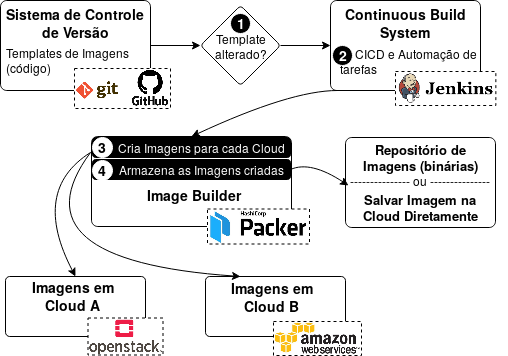
\includegraphics[width=0.7\linewidth]{figuras/Figure2.png}
    	\caption{legenda longa figura2}
    	\label{fig:figure2}
    \end{figure}
    
	O objetivo do processo da Figura2 é prover imagens binárias de servidores que estão dentro dos padrões para rodar em qualquer Nuvem IaaS que fazem parte da Multi-nuvem.
	
	Este processo de criação padronizada de imagens pode alcançar seus objetivos utilizando produtos open-source. Os referenciados na Figura2 são; \textbf{Spinnaker} (http://www.spinnaker.io) que é uma plataforma para entrega contínua (\textit{Continuous Delivery}) de \textit{releases} de software em ambiente Multi-nuvem. \textbf{Packer} (https://www.packer.io) é um framework capaz de produzir multiplas imagens em formatos diferentes, apropriadas para a maioria dor provedores de Nuvem (Públicas e Privadas). Packer pode ser usado com uma variedade grande de \textit{build systems}, dentre os quais destacamos o \textbf{Jenkins} (https://jenkins.io).

	O processo ilustrado na Figura2 é iniciado a partir de um \textit{commit} no \textbf{Sistema de Controle de Versão} em alguma \textit{branch} (Master por exemplo) que é monitorada pelo \textbf{Continuous Build System (1)}. Sempre que uma alteração é feita, o Jenkins executa as rotinas \textbf{(2)} que são requisitos para que o Packer (principal software do \textbf{Image Builder}) possa gerar as imagens de acordo com os \textit{blueprints} de cada Nuvem \textbf{(3)}. O Packer pode armazenar essas imagens para uso futuro em um repositório centralizado (\textit{on-premises} geralmente) ou pode também gravar cada imagem na respectiva Nuvem \textbf{(4)}, essa última alternativa pode ser mais rápida na hora de criar uma instância, pois não precisa fazer a transferência (via Internet) da Imagem armazenada on-premises para a Nuvem.
	
	\section{Validação Experimental - Deployment de aplicação em Multi-nuvem}
	
	Uma das maneiras de experimentar e explorar o processo de deploy de IaaS ou PaaS em Multi-nuvem pode ser feito através do uso de alguns softwares que automatizam a criação de recursos em Nuvem. O uso das consoles WEB ou SDKs disponibolizadas pelos principais provedores de Nuvem, podem ser usados para alguns casos de uso, mas, de forma geral,  propiciam maior chance de erro humano, requerem que a documentação seja feita adicionalmente (geralmente nas fases conclusivas dos projetos) e não aproveitam os benefícios da Infraestrutura como Código (IaC), discutidos anteriormente.
	
	Existem diversas ferramentas que trabalham sob o conceito de IaC e que atendem os requisitos para criação de infraestrutura em Multi-nuvem, uma delas um serviço nativo do Openstack, o Heat, que interage com a API do Openstack para criação ou modificação de Infraestrutura. Heat também consegue atuar em AWS, mas alguns recursos de Infraestrutura ainda não estão definidos no Heat, e, portanto o seu escopo de atuação, para AWS especificamente ainda é muito restritivo, fazendo com que Heat não seja usado em ambientes de produção corporativos. 
	
	Outras ferramentas, tais como Chef, Puppet, Ansible e SaltStack que são muito utilizadas, inclusive em ambientes produtivos, para gerenciamento de configuração de servidores também podem ser usados para criação de recursos e infraestrutura em Nuvens públicas ou Privadas. Estes softwares, entretanto, dependem de módulos, bibliotecas ou outros softwares adicionais para interagirem com as APIs das diversas nuvens suportadas por essas ferramentas. Outro fator limitante é que, nuvens com menor expressividade no mercado tendem a ter menor suporte por parte dessas ferramentas.
	
	Há ainda outra forma de interagir com as APIs das Nuvens, que é via Software Development Kit - SDK (por exemplo, a AWS utiliza boto3, em Python) e cada provedor de Nuvem disponibiliza seu próprio SDK e eles geralmente diferem muito entre si, o que implica que o SDK de uma Nuvem não pode ser usado em outra.
	
	Das soluções listadas acima, podemos notar algumas características que podem ser limitações para uso em produção em ambientes de Multi-nuvem. Os SDKs da maioria dos provedores de Nuvem atende apenas as especificações de API do respectivo provedor de Nuvem (assim como outras ferramentas, como o CloudFormation, que atende somente AWS) e portanto não são boas soluções para gerenciar Multi-nuvem com IaC, pois, não favorecem a fácil replicação de implementações, o reaproveitamento de código, bem como sua manutenção e suporte. Como descrito anteriormente, a maioria dos provedores de Cloud não oferecem APIs padronizadas, dificultando muito o desenvolvimento de ferramentas agnósticas. As ferramentas como Chef, Puppet, Ansible e SaltStack têm foco no gerenciamento de confiração de servidores e não oferecem bom suporte e escopo para criação de infra em múltiplos provedores de Nuvem \cite{Morris:2016}.
	
	Para gerenciar múltiplas Nuvens simultaneamente, é preciso que o Software possa interagir com as diversas APIs dos provedores de Nuvens (públicas ou privadas) e que conte com suporte o mais amplo possível ao gerenciamento dos recursos das Nuvens. Além disso, é importante que a solução tenha constante manutenção e atualizações, em especial a inclusão (rápida) das novas funcionalidades ou serviços que os provedores venham a lançar, tal característica pode ser medida (e eventualmente usada como critério de comparação com outras ferramentas) pela atividade e quantidade de contribuidores do GitHub, por exemplo. De forma complementar, pode-se desejar que a ferramenta tenha uma estrutura de suporte técnico formal (pago) para atender à necessidade (eventualmente regulatória) de algumas corporações.
	
	Durante a pesquisa para este estudo de caso, identificou-se o Terraform, que é uma solução open-source específica para a criação de infraestrutura em Nuvem (dentro do modelo IaC), como uma promissora possibilidade para atender os principais requisitos descritos anteriormente. Diferentemente de ferramentas como o CloudFormation ou os SDKs, o Terraform é uma solução agnóstica, permitindo-lhe criar infraestrutura em praticamente qualquer ambiente, seja ele em Nuvem (Amazon AWS, Microsoft Azure, Google GCP, IBM Cloud, Digital Ocean, etc.), ambiente virtualizado, local ou em Data Centers (VMWare, Xen, Virtual Box, etc.), Docker, Kubernetes, além de recursos diversos de infraestrutura e softwares, tais como Redes (F5 BIG-IP, Palo Alto Networks,etc.), bancos de dados (MySQl ou PostgreSQL), dentre outras (ver www.terraform.io). Terraform conta com uma sólida e ativa comunidade de contribuidores (https://github.com/hashicorp/terraform) e a Hashicorp, empresa que criou o Terraform, oferece suporte, consultorias e treinamento com foco no mercado corporativo.
	
	Na seção a seguir utiliza-se o Terraform para fazer o provisionamento de um servidor com uma aplicação web de teste em duas Nuvens; Openstack e AWS, com o intuito de verificar se o código desenvolvido para os dois provedores atende aos requisitos e características da IaC, conforme listados e discutidos anteriormente.  
	
	\subsection{Validação Experimental com Terraform}
		
	Em https://github.com/arielfrozza/multi-cloud estão disponibilizados os arquivos de código que foram utilizados para a experimentação deste estudo de caso, e que fazem o \textit{deploy} de uma aplicação WEB simples em duas nuvens diferentes; AWS e Openstack. Esse senário tem o objetivo de representar o uso de um caso particular de Multi-nuvem, que é a Nuvem híblida. A execução desses códigos pode ser feita mediante instalação do Terraform em host com acesso às duas Nuvens, e deve-se ter também as credenciais necessárias para a criação de instâncias. Os detalhes dos códigos e sua implementação não serão descritos neste artigo, mas os detalhes e passo a passo encontram-se no repositório do GitHub abaixo dos diretórios openstack\_tf e aws\_tf, para cada uma das duas Nuvens.
	
	O Terraform utiliza como \textit{input} um conjunto de arquivos contendo a definição da infraestrutura, escrita em uma linguagem própria do Terraform, a ser criada nas duas Nuvens. A arquitetura dessa validação segue o modelo apresentado na Figura~\ref{fig:figure1}, mas não de forma integral. O interesse deste estudo é apenas verificar e identificar as vantagens e também as limitações do uso de tal solução à luz dos conceitos de IaC definidos anteriormente, para tal, é criada uma instância Ubuntu 18.04 em cada uma das Nuvens seguido de instalação de alguns softwares (Python 2.7 e Flask) e \textit{deploy} de um código HTTP RESP simples (escrito em Flask).
	
	Desta forma, não serão abordadas nem discutidas as etapas de Telemetria	(e as métricas ou SLAs envolvidos), Pipeline de Imagens, Cofre de Senhas ou Registro de Serviço e Inventário. Processos indicados pelos números 1, 3, 4, 5 na Figura~\ref{fig:figure1}.
	
	A estrutura de código do Terraform (conforme documentada em www.terraform.io/guides) é bem estruturada e pode ser segmentada, permitindo que o código seja dividido em múltiplos arquivos para melhor organização e manutenção. A Figura~\ref{fig:figure3a} lista os arquivos utilizados para este estudo e que estão disponíveis no GitHub. Os arquivos de extensão ".tf" e ".tfvars" contém o código Terraform que interage com as Nuvens para a execução das rotinas. Consta ainda, nestes diretórios, a aplicação de teste, em Flask (simple\_app.py) e o par de chaves (mykey e mykey.pub) para a conexão remota via SSH com as instâncias criadas nas duas Nuvens.  
	
	\begin{figure}[ht]
		\centering
		
\includegraphics[width=0.45\linewidth]{figuras/Figure3a.png}
		\caption{legenda longa figura3a}
		\label{fig:figure3a}
	\end{figure}
	
	O fato de os dois diretórios ilustrados na Figura~\ref{fig:figure3a} terem a mesma estrutura e relação de arquivos, é importante do ponto de vista da IaC, pois, essa característica, facilita a criação e atualizações de documentação e procedimentos operacionais e também pode possibilitar o reaproveitamento de estruturas inteiras ou de blocos de código, e ainda, a manutenção e o controle de versões e mudanças fica facilitado com a segmentação em diferentes arquivos com funções melhor definidas.  
	
	Entretanto, ao fazer a comparação do conteúdo de cada arquivo do Terraform (os ".ft" especialmente) é possível observar facilmente que os códigos diferem substancialmente, conforme ilustrado nas Figura~\ref{fig:figure3b} e Figura~\ref{fig:figure3}, em que, apesar da estrutura e quantidades de arquivos de código escritos para as duas Nuvens serem iguais, devido ao funcionamento do Terraform, a sintaxe para a criação de recursos pode mudar bastante dependendo do provedor de Nuvem em uso, por exemplo, o método de autenticação são essencialmente diferentes para as duas Clouds utilizadas neste estudo, o Openstack requer um usuário com senha e também a URL do Keystone, a região e o domínio utilizado, já a AWS requer apenas a chave de acesso e a \textit{secret key} para fazer a autenticação e autorização, conforme ilustrado na Figura~\ref{fig:figure3b}. 
		
	\begin{figure}[H]
		\centering
		
\includegraphics[width=0.82\linewidth]{figuras/Figure3b.png}
		\caption{legenda longa figura3b}
		\label{fig:figure3b}
	\end{figure}
	
	Outro exemplo dessa diferença de sintaxe também pode ser observada na Figura~\ref{fig:figure3} em que apenas um trecho do código que provisiona as VMs é exibido, mas que mostra claramente que as instruções do Terraform para as duas Nuvens em estudo, diferem muito entre si.
		
	\begin{figure}[ht]
		\centering
		
\includegraphics[width=0.97\linewidth]{figuras/Figure3.png}
		\caption{legenda longa figura3}
		\label{fig:figure3}
	\end{figure}

    o que acabou causando que todos os arquivos diferissem parcialmente de uma Nuvem para outra, conforme Figura~\ref{fig:figure3}, o que dificulta o controle e reuso direto de código.
	
	Durante o desenvolvimento dos códigos, pudemos obter grandes vantagens com o uso do GitHub para controle de versões e mudanças no código, que pode ser testado com mais frequência, a cada incremento no código. Também a documentação ficou mas robusta e coerente, pois, a cada novo \textit{commit} feito, as anotações de comentário eram obrigatórias e síncronas.
	
	Por outro lado, o reuso ainda pode ser feito mediante poucos ajustes. No caso te termos que replicar essa inplementação em um terceiro provedor de Nuvem (Google GCP ou Azure, por exemplo) teríamos apenas que incluir ou retirar algumas linhas específicas para aquela Nuvem e mudaría-mos os valores e nomes das variáveis. Toda a estrutura, relação e quantidade de arquivos permaneceria igual às outras. 
	
	Em nenhuma etapa da escrita ou execução dos códigos tivemos que interagir ou escrever código que interagisse diretamente com as APIs das Nuvens em estudo, isso nos facilitou a escrita e documentação dos códigos.
	
	No caso de uso das SDKs (ou outros serviços como Heat e CloudFormation) das Nuvens, todo o código seria diferente e nada poderia ser reaproveitado para um provedor de Nuvem diferente. 		
	
	\section{Conclusão}
	
	- Usar uma solução agnóstica como Terraform, facilita o estabelecimento de processos padronizados e estruturados de desevolvimento de código e possibilita melhor interação e troca de conhecimento e experiências entre pessoas e times.
	
	- multi nuvem é uma ótima solução para que empresas obtenham fault-torerance, performance, security and cost efficiency para suas ofertas de serviço na Web.
	
	- Há diversas soluções para IaC em Nuvem Pública ou Privadas, mas poucas são agnósticas, completas e robustas o bastante para atender as necessidades de empresas que utilizam multi-nuvem.
	
	- Na validação experimental pudemos observar que o versionamento de código com ferramentas como Git são fundamentais para IaC e que o Terraform se mostrou uma solução agnóstica muito boa para trabalharmos em muti-cloud com IaC.
	
	- O uso de SDKs ou outras soluções, como Heat ou CloudFormation, específicas para provedores de Nuvem específicos dificulta ou impossibilita o reaproveitamento de código e a replicação de implementações entre provedores de Nuvem diferentes. No caso de uso para multi-nuvem com grande numero de provedores participantes, o uso de SDKs e ferramentas específicas pode gerar muita dificulde de controle para manutenção, testes e implementação dos códigos.
	
	- Os principais provedores de nuvem parecem se proteger do mercado em multi-nuvem por não aderirem a padrões de Nuvem API, como as propostas por OASIS, a qual o OpenStak é uma das poucas aderentes.
	
	- A concorrência em alguns setores de serviçõs Web e a crescente exigência do usuário final de serviços de alta qualidade (rápidos, disponíveis e baratos) pode impulsionar alguns setores para o uso de multi-nuvem.	
	
	%Current solutions and their limitations.
	%Problem statement.
	%Solution methodology.
	%Expected contributions.
	%Assumptions and objectives for supporting open-source multi-cloud deployment.
	%Key challenges while deploying enterprise computing in Multi-Cloud Environment.
	%Open-source Multi-Cloud deployment solution framework.
	%Solution to major multi-cloud challenges.
	
	% \textbf{Texto negrito}. Seleciona e CTRL + b
	% \textit{Text itálico}. Seleciona e ctrl + i
	% \textbf{\textit{Text negrito e itálico}}
	% \underline{Text undeline} 
	
	% \begin{flushleft}
	%	Texto à esquerda
	% \end{flushleft}
	
	% \begin{center}
	%	Texto centralizado.
	% \end{center}
	
	% \begin{flushright}
	%	Texto à direita.
	% \end{flushright}
	
	% {\tiny Texto pequeno.}
	% {\LARGE Texto Grande.}
	% Texto Normal.
	
	% \part[test]{title}
	
	% \colorbox{gray}{\textcolor{green}{fundo em cinza com texto verde}}
	% \pagecolor{blue}
	
	\nocite{Bond:2015}
	
	\newpage
	%\bibliographystyle{alpha}
	%\bibliographystyle{plain}
	%\bibliographystyle{unsrt}
	%\bibliographystyle{abbrv}
	%\bibliographystyle{apalike}
	\bibliographystyle{sbc}	
	\bibliography{artigo_multicloud.bib}
	
\end{document}
